\documentclass[a4paper,12pt]{article}
\usepackage[hidelinks]{hyperref}
\usepackage[backend=bibtex]{biblatex}
\addbibresource{biblio.bib}
\usepackage{float}
\usepackage{graphicx}
\usepackage{listings}
\usepackage[utf8]{inputenc}
\usepackage{etoolbox}
\usepackage{fullpage}
\renewcommand*\contentsname{Indice}
\renewcommand*\figurename{Fig.}
\usepackage{setspace}
\usepackage{parskip}
\usepackage{subfigure}
\usepackage{amsmath}
\usepackage{blindtext}
\usepackage{enumitem}


\makeatletter
\patchcmd\l@section{%
  \nobreak\hfil\nobreak
}{%
  \nobreak
  \leaders\hbox{%
    $\m@th \mkern \@dotsep mu\hbox{.}\mkern \@dotsep mu$%
  }%
  \hfill
  \nobreak
}{}{\errmessage{\noexpand\l@section could not be patched}}
\makeatother

\setcounter{secnumdepth}{0}

% un po' di estetica...
\usepackage{fancyhdr}
\pagestyle{fancy}
\setlength{\headsep}{0.35in}
\let\MakeUppercase\relax

% blocchi di codice
\usepackage{listings}
\lstset{
	breaklines=true, 
	frame=single, 
	numbers=left,
	tabsize=2,
	basicstyle=\scriptsize,
	showstringspaces=false
}

\setlength{\parindent}{2em}
\setlength{\parskip}{0.5em}
\renewcommand{\baselinestretch}{1.5}

\fancyhf{} % clear all fields
\fancyfoot[C]{\thepage}

\frenchspacing

\begin{document}

\begin{titlepage}
\noindent
    \vspace*{5mm}
	\begin{minipage}[t]{0.15\textwidth}
	    \vspace*{5mm}
		\vspace{-3.5mm}{
\includegraphics[scale=1.8]{img/logo_bicocca.png}}
	\end{minipage}
	\hspace{1cm}
	\begin{minipage}[t]{0.9\textwidth}
	      \vspace*{5mm}
		{
			\setstretch{1.42}
			{\textsc{Università degli Studi di Milano - Bicocca} } \\
			\textbf{Scuola di Scienze} \\
			\textbf{Dipartimento di Informatica, Sistemistica e Comunicazione} \\
			\textbf{Corso di Laurea Magistrale in Informatica} \\
			\par
		}
	\end{minipage}
	
	\vspace{42mm}

\begin{center}
    {\LARGE{
	    	\setstretch{2}
            \textbf{
            	Sperimentazione Record Linkage \\ }
    }}        
\end{center}

\vspace{40mm}
	
	
	\begin{flushright}
		\setstretch{1.3}
		\large{Alberici Federico - 808058\\} 
		\large{Bettini Ivo Junior - 806878\\} 
		\large{Cocca Umberto - 807191\\} 
		\large{Traversa Silvia - 816435} 
	\end{flushright}
	
	\vspace{15mm}
	\begin{center}
		{\large{\bf Anno Accademico 2019 - 2020}}
	\end{center}


\renewcommand{\baselinestretch}{1.5}

\end{titlepage}

\tableofcontents

\newpage

\section{Ricerca preliminare} 

\subsection{Data Quality}

La consapevolezza del peso che dati di alta qualità hanno nel supportare decisioni informate e, viceversa, delle conseguenze disastrose cui dati inaccurati possono portare, è cresciuta di pari passo con il diffondersi delle fonti informative a disposizione delle organizzazioni, creando sempre più forte l’esigenza di una gestione adeguata della qualità dei dati aziendali. La ricerca sulla qualità dei dati è iniziata correttamente negli anni '90 e varie definizioni di ciò sono state date nel corso degli anni. \\

\noindent Un gruppo di ricerca del MIT, guidato dal professor Wang, ha definito la qualità dei dati come condizione per il loro utilizzo e ha proposto il loro giudizio dipendentente dai consumatori finali. Allo stesso tempo, hanno definito una "dimensione della qualità dei dati" come un insieme di attributi che rappresentano un singolo aspetto o costrutto della qualità dei dati. \\

\noindent Sono necessarie tecniche di misurazione completa per consentire alle organizzazioni di valutare lo stato della qualità delle informazioni organizzative e monitorarne il miglioramento. \\

\noindent Ma cosa si intende quando si parla di qualità dei dati e come si misura? 
La qualità dei dati è una caratteristica che ha a che fare con la loro abilità di soddisfare le esigenze e le aspettative implicite o esplicite dell'utente. 

\noindent Le best practice in questo ambito suggeriscono l’utilizzo di opportune metriche per la definizione e la misurazione della qualità dei dati. 

\noindent Per quanto riguarda la definizione di metrica ci riferiamo alle definizioni all'interno dello standard ISO 9126-1 e framework ISM3:
\begin{itemize}
	\item una procedura (o metodo) di misurazione, cioè un algoritmo che prende l'elemento per misurare e lo associa a misura (sia esso valore ordinale o intervallo); 
	\item una corretta unità di misura (o scala), ovvero di dominio di valori restituiti dalla procedura di misurazione. In generale, è possibile associare diverse metriche a ciascuna dimensione di qualità;
\end{itemize} 
Questa può essere espressa attraverso molteplici dimensioni

Tra le metriche più comuni troviamo:

\begin{itemize}
\item \textbf{completezza}: i dati raccolti bastano per rappresentare l'informazione necessaria; 
\item \textbf{accuratezza}: la precisone dei dati;
\item \textbf{tempestività}: i tempi di acquisizione dei dati sono utili per il processo;
\item \textbf{coerenza}: i dati non sono contradditori tra di loro;
\item \textbf{univocità}: i dati rappresentativi della stessa informazione presenti in diversi componenti del sistema informativo assumono lo stesso valore;
\item \textbf{integrità}: i dati presenti nel sistema informativo corrispondono a quelli originariamente immessi;
\item \textbf{conformità formale}: i dati immessi nel sistema informativo rispettano gli standard formali appositamente definiti.
\end{itemize} 

\bigskip

\noindent Il punto focale rimane sempre il dominio sul quale si vuole effettuare un processo di miglioramento dei dati. In base alla finalità delle informazioni e alle caratteritiche dei loro consumatori l'attenzione si rivolge ad un sottoinsieme di tale metriche.\\
In tempi attuali, è emerso un altro tipo problema: i big data. Analisi e ricerca complete di standard di qualità e metodi di valutazione della qualità per questo tipo di informazioni attualmente è assente o non completa. Questo topic pone una serie di nuove sfide, dettate dalle caratteristiche intrinseche dei big data, riassumibili in quelle che sono chiamate "le 5 V":
\begin{itemize}
	\item \textbf{Volume}: ingente massa di informazioni, in crescita vertiginosa, che non è possibile raccogliere con tecnologie tradizionali;
	\item \textbf{Velocity}: i dati nascono e vengono acquisiti sempre più rapidamente, con necessità di analisi in tempo reale;
	\item \textbf{Variety}: differenti tipologie di dati disponibili, provenienti da un numero crescente di fonti eterogenee;
	\item \textbf{Veracity}: i dati devono essere affidabili, raccontare il vero;
	\item \textbf{Value}: abilità di trasformare una grande mole di dati in business.
\end{itemize}

\subsubsection{Metodologia Data Quality}

Il professor Batini definisce la metodologia di qualità dei dati come un insieme di linee guida e tecniche che, a partire dalle informazioni di input che descrivono un determinato contesto applicativo, ne deriva un processo razionale per valutare e migliorare la qualità dei dati \cite{10.1145/1541880.1541883}. Ci sono tre fasi principali per tale attività:
\begin{itemize}
\item \textbf{ricostruzione dello stato}, al fine di ottenere due informazioni contestuali, facoltative se sono già disponibili per l'uso;
\item \textbf{valutazione e misurazione}, misurazione della qualità lungo dimensioni della qualità pertinenti o valutazione, quando tali misurazioni vengono confrontate con i valori di riferimento;
\item \textbf{miglioramento}, attività che mirano per raggiungere nuovi obiettivi di qualità dei dati.
\end{itemize}

\subsubsection{Miglioramento}

Il miglioramento della qualità dei dati può essere effettuato attraverso strategie basate sui dati o sui processi. Nel primo caso, le tecniche più diffuse sono quella di standardizzazione (o normalizzazione), di record linkage e di integrazione degli schemi e dei dati, mentre nel secondo caso si adotta un processo di ricostruzione. Nel caso del nostro progetto, per poter migliorare la qualità del dato abbiamo deciso di utilizzare la tecnica del record linkage, in quanto ci siamo trovati di fronte ad una grande quantità di dati proveniente da diverse fonti e con informazioni non uniformi fra di esse.

\subsubsection{Standardizzazione}

Questo processo, chiamato anche \textit{normalizzazione}, sostituisce per esempio una diversa ortografia di una parola con una sola ortografia. % e basta?

\subsubsection{Comparazione stringhe}

Gli errori tipografici rendono impossibile confrontare esattamente tra di loro le stinghe.  Per poter fare ciò, quindi, serve una funzione che cerca di trovare un punto di accordo tra i dati. Ci sono stati diversi tentativi di fornire questa funzione:

\begin{itemize}
\item Jaro \cite{census/jaro76} nel 1976 ha proposto un comparatore di stringhe che tiene conto di inserimenti, eliminazioni e trasposizioni necessarie per abbinare le due stringhe;
\item Winkler \cite{winkler90} nel 1990 ha proposto una variante della distanza Jaro (Jaro-Winkler);
\item la distanza q-gram conta il numero di q caratteri consecutivi che concordano tra due corde;
\item la distanza di edit classica, che conta il numero di operazioni (inserimenti, eliminazioni, modi cazioni) necessarie per abbinare le due stringhe
\end{itemize}

\subsection{Record Linkage}

Il record linkage (conosciuto anche come data matching) è l'operazione che consiste nel trovare "records" che si riferiscono alla stessa entità, in dataset presi da differenti risorse (come ad esempio file, libri, siti e database). 
Questa operazione diventa necessaria quando vogliamo unire dei dataset differenti basati su dati simili che potrebbero avere o non avere lo stesso identificativo. \\
L'idea moderna di record linkage nasce alla fine degli anni cinquanta e viene formalizzata qualche tempo dopo da Ivan Fellegi e Alan Sunter \cite{fellegi69} che, attraverso il loro lavoro, hanno dimostrato che le regole di decisione probabilistiche sono ottimali quando i dati che vengono confrontati sono condizionatamente indipendenti. \\
A partire dalla fine degli anni novanta, differenti tecniche di machine learning sono state sviluppate per poter capire, con condizioni favorevoli, la probabilità condizionata richiesta dalla teoria Fellegi-Sunter. \\
Il record linkage può essere interamente eseguito senza l'aiuto di un computer, ma il motivo principale per cui esso viene utilizzato è perchè si vuole ridurre o eliminare le modifiche "fatte a mano" e per rendere più facile l'ottenimento del risultato. 
%aggiungere qualcosa guardando magari l'articolo di Batini?
\\

\noindent Il record linkage si divide generalmente nei seguenti step:
\begin{enumerate}
\item vengono dati in input dei dataset;
\item viene definito uno spazio iniziale di ricerca;
\item si cerca di ridurre lo spazio di ricerca tramite un processo di "blocking" ;
\item viene definito lo spazio ridotto di ricerca;
\item vengono comparati i dati e viene presa una decisione;
\item vengono definitie le regole di matching, possibile matching o non-match;
\item secondo le regole definite viene generato il dataset di output.
\end{enumerate}

\begin{figure}[H]
	\centering
	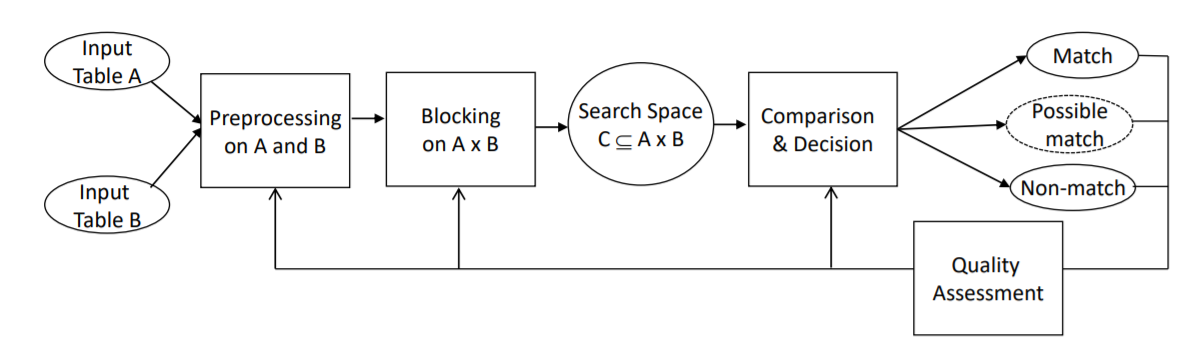
\includegraphics[width=0.8\linewidth]{img/recordlinkage.png}
	\caption{\textit{Step principali del record linkage}}
\end{figure}

\newpage
\subsubsection{Metodologie record linkage}

\begin{description}[align=left]
	\item[Data preprocessing] Il record linkage è molto sensibile alla qualità dei dati che devono essere collegati, quindi idealmente prima di svolgere questa operazione ogni dataset deve essere controllato affinche la qualità sia delle migliori. Avvengono delle operazioni di standardizzazione, che consistono nel trasformare i dati o procedure più complesse, come ad esempio la tokenizzazione.
	\item[Entity resolution] L'entity resolution è un processo di operazioni intelligenti che permettono alle organizzazioni di connettere i dati più disparati attraverso la possibilità di capire i matches tra le entità e le relazioni non ovvie fra i diversi dati.\\Essa analizza tutte le informazioni collegate ad una entità prese da diverse sorgenti e cerca, attraverso un calcolo probabilistico, di determinare quali entità sono collegate e quali collegamenti (non ovvi) esistono fra loro.
	\item[Deterministic record linkage] La metodologia più semplice di record linkage è chiamata "deterministica".\\Essa genera collegamenti basati sul numero di singoli identificatori che hanno una corrispondenza fra i dati dei dataset.\\Due record si dicono \textit{collegati} con una procedura di record linkage deterministico se se tutti o alcuni degli identificatori sono identici.\\Questo metodo è una buona opzione se si stanno utilizzando dei dataset con delle entità che sono identificate da un id comune.
	\item[Probabilistic record linkage] Il record linkage probabilistico, chiamato anche \textit{fuzzy matching}, utilizza un approccio differente per poter collegare i dati. Viene tenuto conto di una gamma più ampia di potenziali identificatori, calcolando i pesi per ciascun identificatore in base alla sua capacità stimata di identificare correttamente una corrispondenza o una non corrispondenza. Questi pesi sono dunque usati per calcolare la probabilità che due dati registrati si riferiscano alla stessa entità.\\Le coppie di record con probabilità al di sopra di una determinata soglia sono considerate corrispondenze, viceversa le altre sono considerate non corrispondenze. Le coppie che rientrano tra queste due soglie sono considerate "possibili corrispondenze" e possono essere trattate di conseguenza (ad esempio, revisioni umane, collegate o non collegate, a seconda dei requisiti). Mentre il collegamento deterministico dei record richiede una serie di regole potenzialmente complesse da programmare in anticipo, i metodi probabilistici di collegamento dei record possono essere "addestrati" per funzionare bene con un intervento molto meno umano.
	\item[Machine learning] Negli ultimi anni, sono state utilizzate varie tecniche di apprendimento automatico per collegamento automatico. È stato riconosciuto che l'algoritmo classico per il collegamento probabilistico dei record sopra descritto è equivalente all'algoritmo Naive Bayes nel campo dell'apprendimento automatico, e utilizza la stessa assunzione dell'indipendenza delle sue caratteristiche (un presupposto che in genere non è vero).\\È possibile ottenere una maggiore precisione utilizzando varie altre tecniche di apprendimento automatico, incluso un percettrone a strato singolo. Insieme alle tecnologie distribuite, l'accuratezza e la scala per il collegamento dei record possono essere ulteriormente migliorate.	
\end{description}

\subsection{Tools}
Di seguito riportiamo i tool e le librerie che abbiamo utilizzato (o tentato di usare) durante il nostro progetto.

\subsubsection{Python Record Linkage Toolkit}
Python Record Linkage Toolkit è una libreria che permette di effettuare record linkage sia in una sola fonte di dati che in multiple.Il toolkit fornisce la maggior parte degli strumenti necessari per il collegamento e la dedpulicaizone dei record.
 Il package contiene metodi di indexing, come blocking e sorted neighbourhood indexing, funzioni per il confronto con diverse misure di similarità possibili e diversi algoritmi di classificazione, sia supervisionati che non. 
Uno degli obiettivi principale è proprio creare un framework estendibile per il collegamento dei record, per fare questo il tool è in grado di:
\newpage
\begin{itemize}
\item pulire e standardizzare i dati
\item creare coppie di record con metodi di indicizzazione intelligente
\item confrontare i record con un gran numero di misure e di comparazione e somiglianza per diversi tipi di variabili
\item utilizzare diversi algoritmi di classificazione
\item valutare, attraverso strumenti comuni, i collegamenti dei record
\end{itemize} 

Per raggiungere l'obiettivo del nostro progetto è stato fondamentale poichè ci permette di svolgere tutte le operazioni del record linkage senza dover ricorrere all'utilizzo di ulteriori tool.

\subsubsection{Pandas}
Pandas è una libreria software scritta in linguaggio python che permette la manipolazione e l'analisi dei dati. L'obiettivo di questo tool è diventare il blocco di base di alto livello fondamentale per eseguire analisi dei dati reali. Inoltre, ha l'obiettivo più ampio di diventare lo strumento di analisi e manipolazione dei dati open source più potente e flessibile disponibile per qualsiasi linguaggio.\\
Questo tool è in grado di pulire, esplorare e elaborare i dati. In Pandas una tabella viene chiamata dataframe, ed è proprio grazie a questo tool che siamo riusciti  creare i due dataframe principali che poi utilizziamo nella fase di record linkage.

\subsubsection{Fuzzy Matcher}
Fuzzy Matcher è un pacchetto python che permette all'utente di collegare due dataframe pandas basati su uno o più campi in comune. Fuzzymatches usano la ricerca del testo completa sqlite3 per trovare dei match potenziali.
% lo  usiamo si o no? se si scrivere perchè, se no scrivere perchè

\newpage
\section{Sperimentazione}

\subsection{Dataset}
Il dataset su cui sono stati effettuati gli esperimenti è un elenco di ristoranti di Manhattan, estratti settimanalmente da Gennaio a Marzo 2009 da 12 siti web. L'unico attributo comune in tutti i dataset è il nome del ristorante, informazioni aggiuntive (come l'indirizzo o il quartiere) non sono presenti in modo uniforme.

\subsection{Analisi dei dati}
I dati sono messi a disposizione in sette file di testo, uno per ogni settimana considerata, ciascuno contenente informazioni appartenenti a tutti i siti web. In totale sono presenti 215555 record, suddivisi come illustrato nella seguente tabella:
\begin{table}[H] \centering
\begin{tabular}{|l|l|}
\hline
\multicolumn{1}{|c|}{\textbf{file}} & \multicolumn{1}{c|}{\textbf{records}} \\ \hline
restaurants\_2009\_1\_22.txt & 30401 \\ \hline
restaurants\_2009\_1\_29.txt & 30775 \\ \hline
restaurants\_2009\_2\_05.txt & 30805 \\ \hline
restaurants\_2009\_2\_12.txt & 30863 \\ \hline
restaurants\_2009\_2\_19.txt & 30876 \\ \hline
restaurants\_2009\_2\_26.txt & 30898 \\ \hline
restaurants\_2009\_3\_12.txt & 30937 \\ \hline
\end{tabular}
\caption{Record presenti nei file txt forniti}
\end{table}

In particolare, per ogni ristorante è presente il seguente numero di record:

\begin{table}[H]\centering
\begin{tabular}{|c|c|}
\hline
\textbf{restaurant} & \textbf{records} \\ \hline
ActiveDiner & 6184 \\ \hline
DiningGuide & 814 \\ \hline
FoodBuzz & 2079 \\ \hline
MenuPages & 13143 \\ \hline
NewYork & 1774 \\ \hline
NYMag & 5124 \\ \hline
NYTimes & 3095 \\ \hline
OpenTable & 1539 \\ \hline
SavoryCities & 4536 \\ \hline
TasteSpace & 3635 \\ \hline
TimeOut & 14007 \\ \hline
VillageVoice & 2684 \\ \hline
\end{tabular}
\caption{Record per ristorante}
\end{table}

E sono presenti le seguenti informaizoni: 
\begin{itemize}
\item \textbf{ActiveDiner}: nome ristorante, indirizzo, paese
\item \textbf{DiningGuide}: nome ristorante, indirizzo
\item \textbf{FoodBuzz}: nome ristorante, indirizzo, paese, codice paese, quartiere, tipo, costo
\item \textbf{MenuPages}:nome ristorante, indirizzo1, indirizzo2
\item \textbf{NewYork}: nome ristrorante
\item \textbf{NYMag}: nome ristorante, quartiere
\item \textbf{NYTimes}: nome ristorante, quartiere
\item \textbf{OpenTable}: nome ristorante, quartiere
\item \textbf{SavoryCities}: nome ristorante, indirizzo, quartiere
\item \textbf{TasteSpace}: nome ristorante, indirizzo, paese
\item \textbf{TimeOut}: nome ristorante, posizione, indirizzo1, indirizzo2, indirizzo3, quartiere, numero di telefono, tipo
\item \textbf{VillageVoice}: nome ristorante, indirizzo, quartiere
\end{itemize}

Possiamo notare che non sono presenti tutte le stesse informazioni in tutti i dataset, cosa che ci ha recato non pochi problema durante la fase di linkage. Per questo motivo il dataset "NewYork" non è stato utilizzato poichè non portava informazione utile.

\subsection{Data preprocessing} 
Una prima analisi mostra come le modalità di recupero dei dati da parte dell'autore abbiano generato dei dataset differenti per schema e per frammentazione verticale, anche sulle stesse fonti. Dunque, prima di applicare le tecniche di record linkage, i dati sono stati standardizzati, eseguendo operazioni di riallineamento dello schema, rimozione dei duplicati ed infine join dei dataset per fonte.\\
La fase di preprocessing, nella quale sono incluse la pulizia dei dati e la standardizzazione, sono importanti poiché potrebbero aumentare l'accuratezza del record linkage.\\
In dettaglio le fasi del preprocessing sono state: % mettere esempi più precisi dei problemi trovati
\begin{enumerate}
	\item \textbf{Separazione e ragruppamento dei dati per fonte}.\\Ciò ha mostrato le differenze sullo schema, utilizzate nelle fasi successive per migliorare il raggruppamento dei dati.
	\item \textbf{Separazione dei dati per fonte e data}.\\Utilizzando regex ad hoc per ogni fonte i dati sono stati separati per fonte e data, con drop dei duplicati, standardizzazione dell'encoding del testo (da \textit{windows-1252} a \textit{UTF-8}) e formato csv.
	\item \textbf{Merge dei dataset per fonte}.\\I vari dataset risultanti dalla fase 2 sono stati riuniti per fonte con un join applicato su colonne definite a priori. 
	\item \textbf{Pulizia finale}.\\I dataset dunque sono stati ripuliti utilizzando delle funzioni specifiche per ogni fonte, con il compito di riallineare lo schema, rimuovere duplicati e caratteri superflui dai valori (es spazi e tabulazioni in testa e in coda, caratteri speciali ecc.).  
\end{enumerate}

\subsection{Google Maps}
Nei vari dataset le informazioni riguardanti l'indirizzo non erano riportare in maniera uniforme (es. \textit{Street} in un record e \textit{St.} in un altro), quindi abbiamo deciso di standardizzare questo parametro ricorrendo alle API di Google Maps.

Come prima cosa abbiammo creato una API key per poter dialogare con le 
\href{https://console.cloud.google.com/google/maps-apis/overview?project=feisty-nectar-281812&folder=&organizationId=}{API di Google} %mettere colore blu


Consultando la \href{https://developers.google.com/places/web-service/search}{documentazione} abbiamo individuato la funzione 
Text Search, la quale è molto simile alla funzione di autocompletamento presente su Google Maps e che quindi ci permette di ricavare indirizzo completi partendo da informazioni parziali.

Pertanto è stato costruito uno script che esegue una GET al seguente \href{https://maps.googleapis.com/maps/api/place/textsearch/json }{indirizzo}, passando come parametro la stringa \textit{address} del record del csv considerato. L'output ottenuto è un json.

% la si può prendere direttamente dal sito di google nella funzione textsearch
% https://console.cloud.google.com/google/maps-apis/overview?project=feisty-nectar-281812&folder=&organizationId=
\begin{figure}[H]
	\centering
	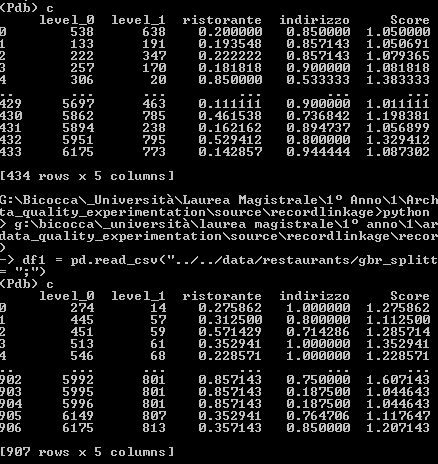
\includegraphics[width=0.8\linewidth]{img/img.png}
	\caption{\textit{Dati dopo il preprocessing di MenuPages}}
\end{figure}

\noindent Il campo da noi considerato è formatted\_address. In caso di indirizzo scritto male o con contenuto informativo ambiguo venivano restituiti più formatted\_address, pertanto si è deciso che se il numero di risultati ottenuto era maggiore di 5 allora non si è applicata tale trasformazione, poiché probabilmente non porterebbe reali benefici. Negli altri casi si è preso solo il primo risultato. 

Nello specifico,  dato che tutti i ristoranti sono a New York, abbiamo splittato la stringa recuperando solo la prima parte (fino alla prima virgola), in quanto l'informazione sulla città è superflua. 
 
%CAMBIARE ESEMPIO PERCHè C'è SCRITTO AUSTRALIA MINCHIA
es preso dall'immagine
140 george st, the rocks Nsw 200m, australia

noi abbiamo preso solo 140 george st

In questo modo facendo i confronti il contenuto informativo era maggiore e non degradato da New york, NY , dati che sarebbero stati comuni a tutti.

\subsubsection{Risultati}
Nel caso di MenuPages, per esempio, inizialmente i dati erano presenti in un txt in questo formato ed erano uniti ai dati di altri siti web:\\
\begin{figure}[H]
\centering
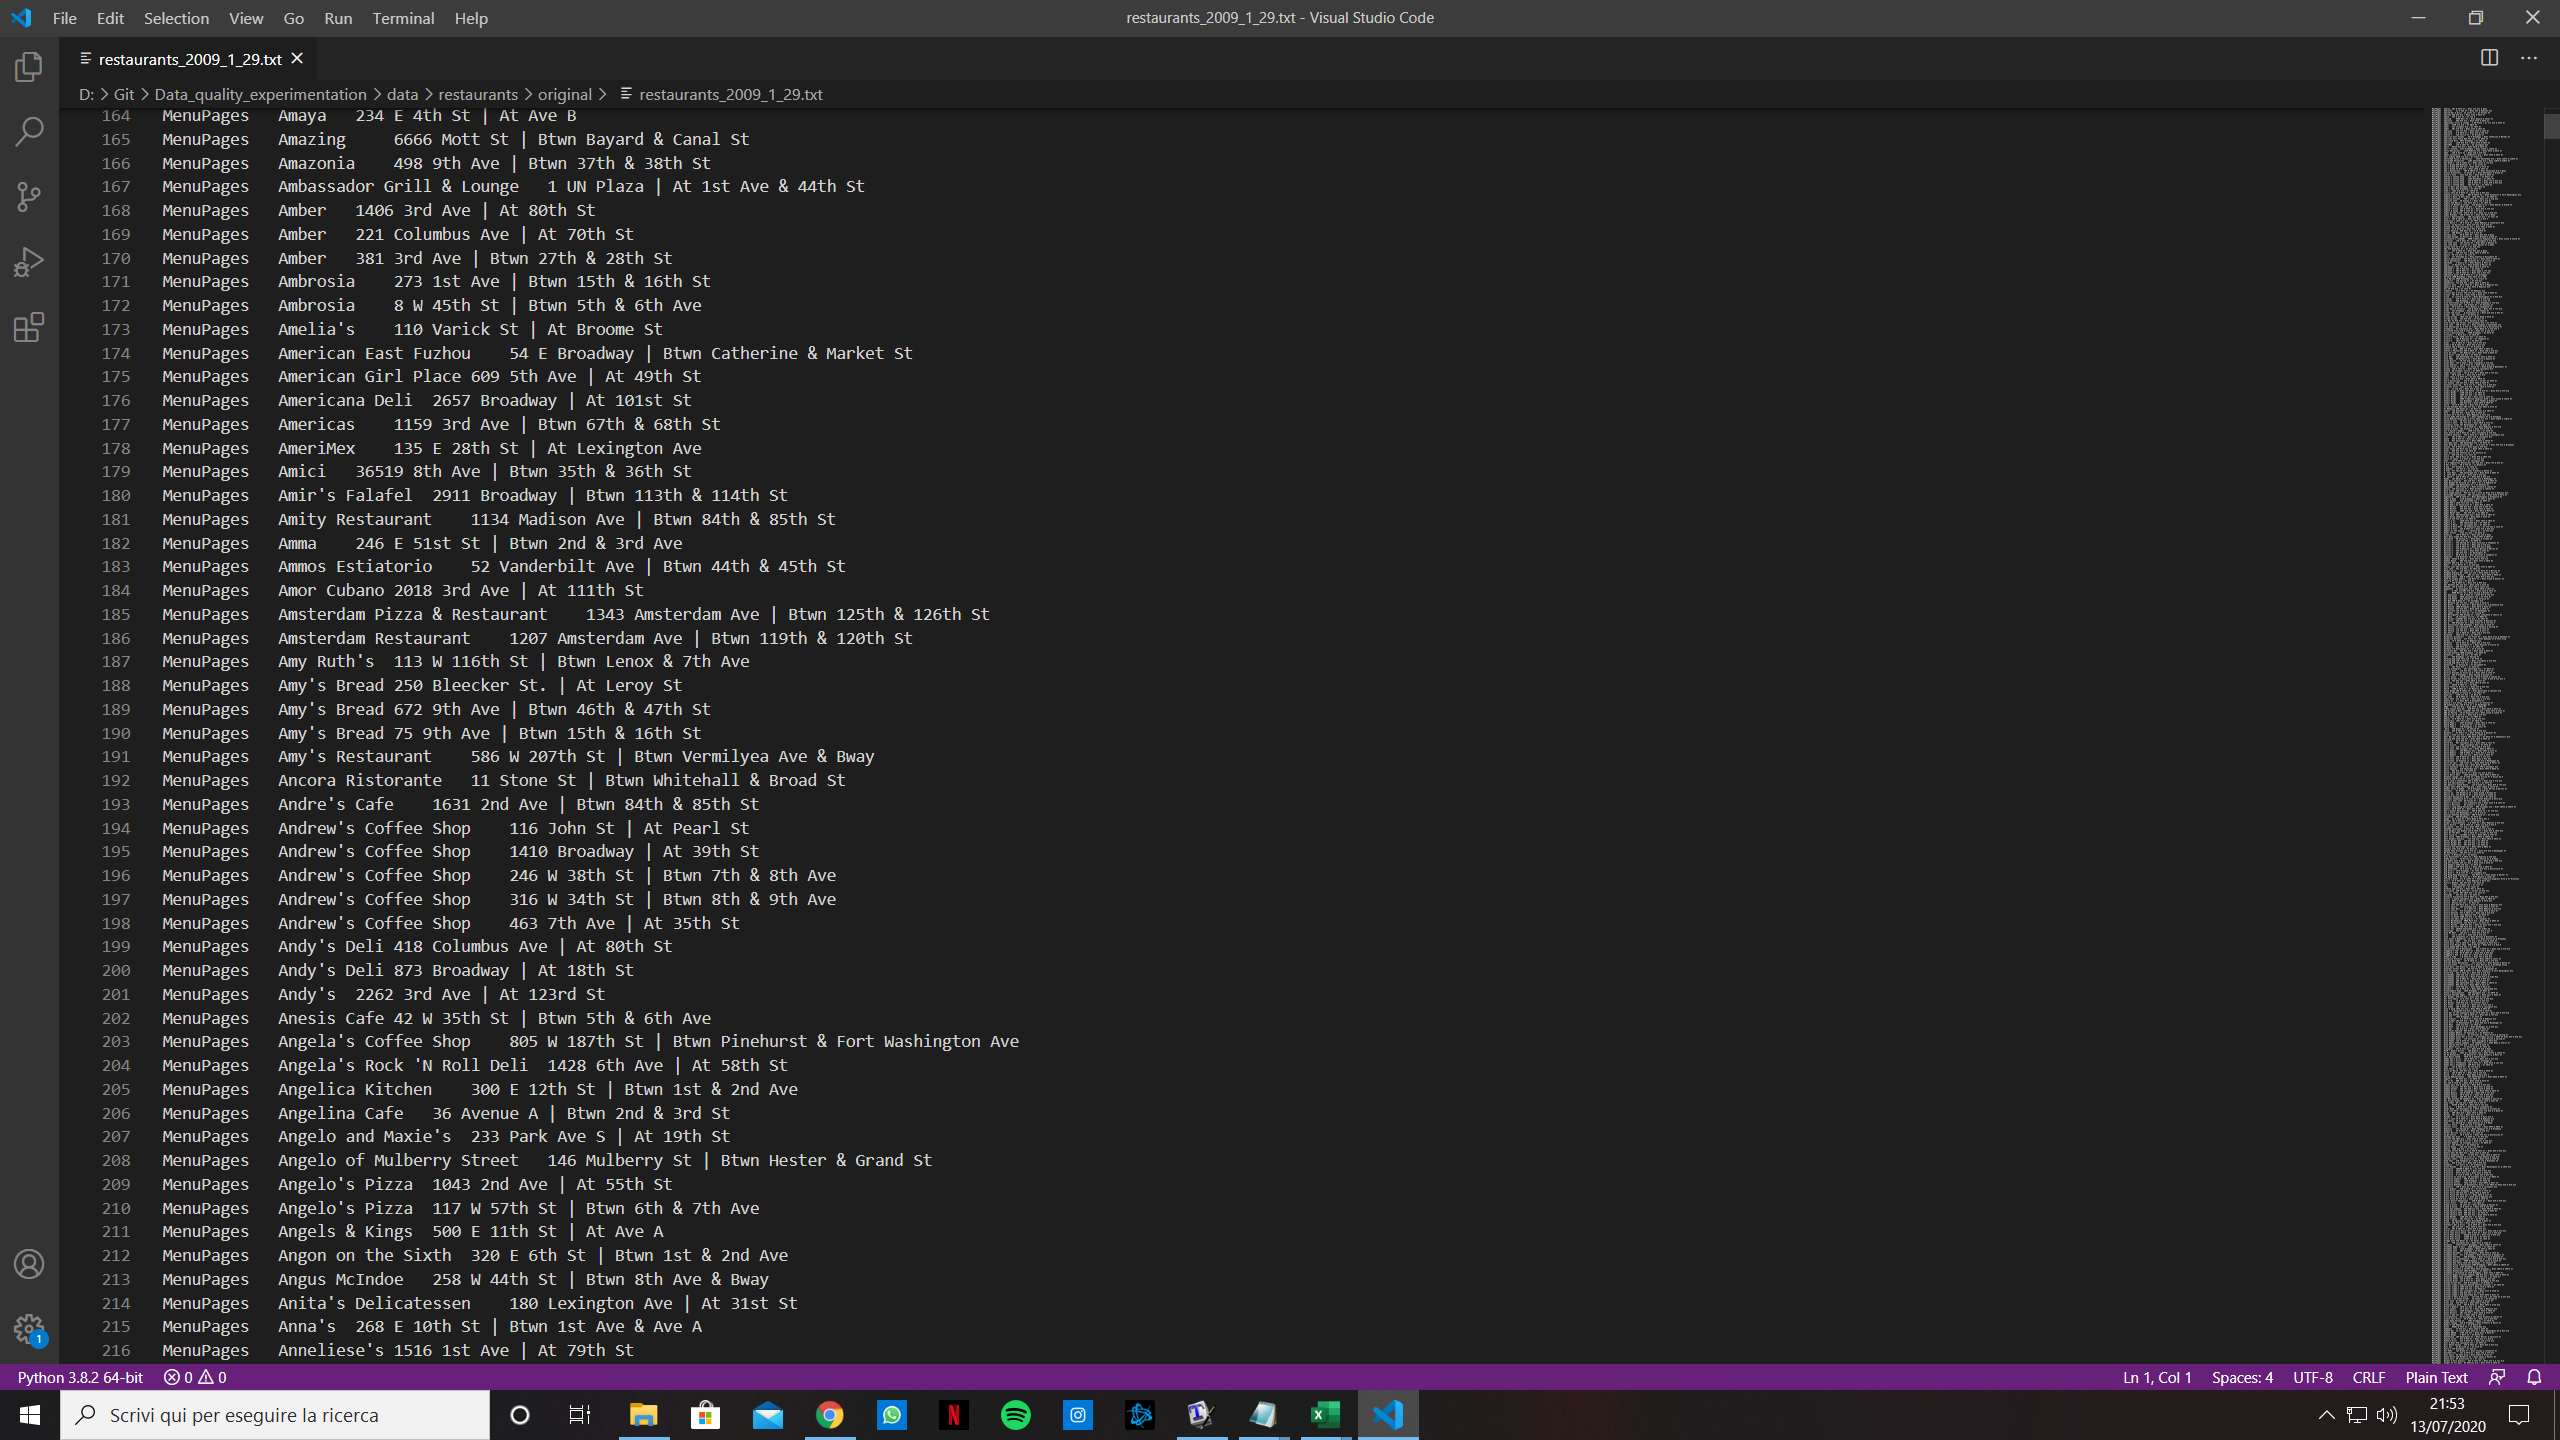
\includegraphics[width=0.65\linewidth]{img/original.png}
\caption{\textit{Dati di partenza di MenuPages}}
\end{figure}

a seguito del preprocessing invece otteniamo informazioni più chiare, aggiungendo l'informazione sull'indirizzo proveniente da Google come segue:\\

\begin{figure}[H]
\centering
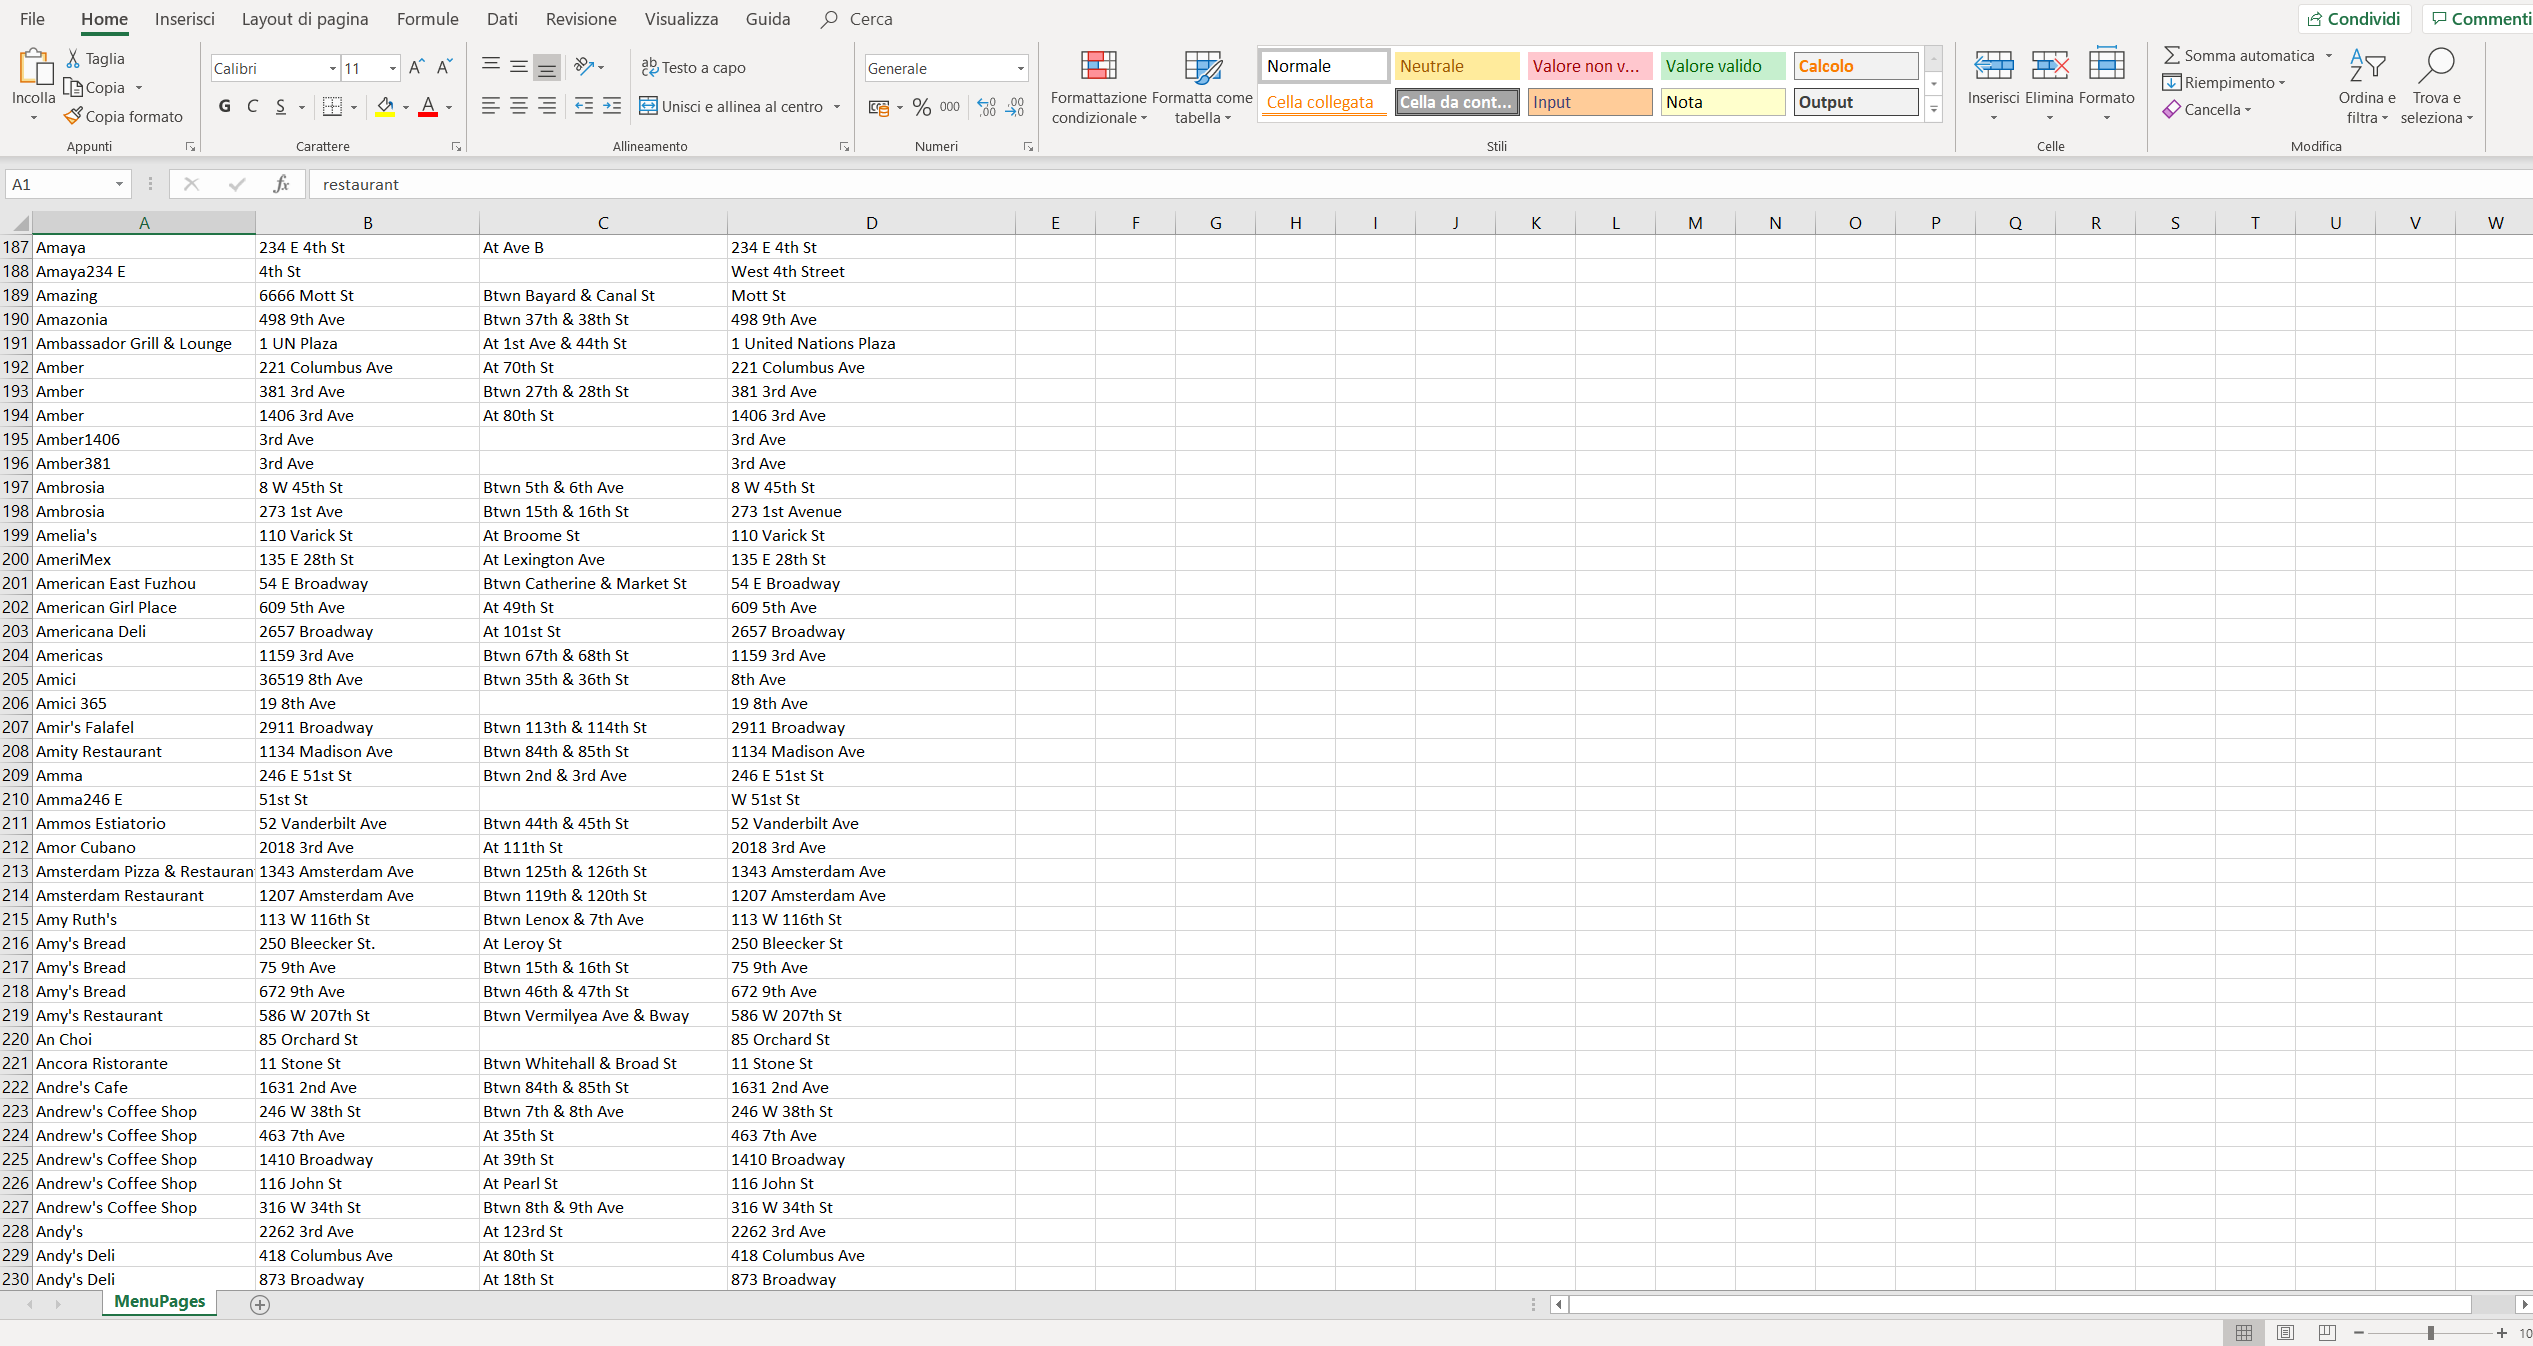
\includegraphics[width=0.65\linewidth]{img/new.png}
\caption{\textit{Dati dopo il preprocessing di MenuPages}}
\end{figure}

\newpage
\subsection{Record Linkage}
Dalla fase di preprocessing abbiamo ottenuto in output 12 dataset, uno per ogni sito web presente nei file originali. Prima di procedere con l'attività di record linkage abbiamo deciso di introdurre una fase preliminare per costruire due dataset principali da poi linkare.

\subsubsection{Fase preliminare: costruzione dataset}
Analizzando i dataset ottenuti siamo riusciti ad individuare delle caratteristiche comuni in grado di distinguerli in due macro gruppi:
Nei dataset \textit{nomi dei dataset presenti in first df generator} %%%%% 
si hanno esclusivamente il nome del ristorante e il quartiere (solo in \textit{TimeOut} abbiamo in aggiunta l'indirizzo, che ci permetterà il linkage con l'altro dataset), nei dataset \textit{nomi dei dataset presenti in second df generator} %%%%% 
, invece, abbiamo nome del ristorante e indirizzo in tutti i file.

Per ogni insieme di dataset, dopo aver uniformato i nomi e l'ordine delle colonne presenti, abbiamo eseguito un append di tutti i dataframe generati importando i file csv. 
Successivamente sono stati rimossi i duplicati presenti basandoci solo sulle colonne comuni per tutti, ossia \textit{restaurant} e \textit{neighbourhood} nel primo caso e \textit{restaurant} nel secondo (non è possibile utilizzare l'indirizzo in quanto non sono sempre scritti esattamente allo stesso modo nonostante rappresentino la stessa realtà) %%controllare

Successivamente viene applicata la \textbf{deduplicazione}, ossia una tecnica usata per eliminare copie duplicate di dati ripetuti. È possibile applicarla attraverso la libreria \textit{Record Linkage Toolkit} in quanto viene vista come un record linkage effettuato tra il database e se stesso. Come tecnica di \textit{indexing} usiamo \textit{sortedneighbourhood} (che illustreremo in dettaglio in seguito) ed effettuiamo la fare di \textit{comparing} sugli attributi comuni nei rispettivi gruppi di dataset.

In questa fase iniziale per classificare i match ci siamo basati esclusivamente sul punteggio di score ottenuto dalla fase di comparing, in modo da poter includere con sicurezza record che differivano solo di poche lettere (ad esempio i ristoranti "Bubba Gump Shrimp Co." e "Bubba Gump Shrimp Company"), scegliendo come valore di soglia dello score %inserire valore.

Una volta individuati i match sono stati unificati i dati in modo da creare un dataframe contenente le informazioni uniche utili per ogni match trovato. Per ottenere il dataset finale dal primo dataframe ottenuto come l'append dei csv importati sono state rimosse tutte le righe delle coppie presenti nei match e sono state aggiunti i record unificati contenenti le informazioni complete.

Da questa fase sono risultati due dataset, rispettivamente di 7524 e di 13379 record, invece dei 58614 %controllare sia giusto by ivo
record totali derivati dall'unione di tutti i 12 file iniziali.

\subsubsection{Fase principale: record linkage}
Per la fase di record linkage abbiamo seguito la seguente pipeline: 
%inserire immagine

I passi principali seguiti sono i seguenti:
\begin{itemize}
\item \textbf{Indexing} - permette di creare coppie di record, denominate \textit{candidate links}. Nel nostro algoritmo abbiamo implementato tre tecniche di indexing: \\
- \textit{full}, che crea le coppie effettuando il prodotto cartesiano dei due dataset, motivo per il quale è molto lungo e sconsigliato. \\
- \textit{blocking}, che permette di creare le coppie basandosi su una o più variabili uguali. \\
- \textit{sortedneighbourhood}, da usare nel momento in presenza di dataset con un grande numero di errori di spelling nei valori.
\item \textbf{Comparing} - viene usato per confrontare le coppie di record create nella fase di indexing, sfruttando diversi metodi di similarità. Nel nostro caso abbiamo effettuato un confronto fra stringhe testando alcuni dei vari metodi disponibili (‘jaro’, ‘jarowinkler’, ‘levenshtein’, ‘lcs’) e impostando un valore di soglia (tutti i confronti approssimativi di stringhe più alti o uguali a questa soglia valgono 1) oppure usato un confronto esatto nel momento in cui trattavamo l'attributo \textit{addressGoogle}, che sappiamo essere uniforme.
\item \textbf{Classification} - dove le coppie vengono classificate in matches, non-matches e possible matches. In particolare abbiamo deciso di applicare due algoritmi di apprendimento non supervisionato, non essendo in possesso di training data. Gli algoritmi adottati sono: \\
- \textit{ECM Classifier} o \textit{Expectation/Conditional Maxisation classifier}, un algoritmo probabilistico dove viene trovata iterativamente la massima probabilità (locale) o la massima stima a posteriori (MAP) dei parametri nei modelli statistici. L'iterazione EM si alterna tra l'esecuzione di un passaggio di aspettativa (E), che crea una funzione per l'aspettativa della verosimiglianza, e un passaggio di massimizzazione (M). \\
- \textit{KMeans Classifier}, algoritmo che suddivide le coppie di record in match e non-match ed ogni vettore di confronto appartiene al cluster con la media più vicina. L'algoritmo è calibrato per due cluster: un cluster di corrispondenza e un cluster di non corrispondenza.
\item {Evaluation} - permette di verificare la qualità del linkage in termini di accuratezza, recall e F-score. Purtroppo non ci è stato possibile eseguire questa fase in quanto sprovvisti di \textit{veri positivi}.
\end{itemize}

\subsubsection{PIPPO}
I dati di addestramento non sono generalmente disponibili nelle applicazioni di record linkage perché sono set di dati specifici del campione, infatti nel nostro caso non sono forniti dei true matches. \\
Python Record Linkage Toolkit fornisce un'interfaccia utente basata su browser per la classificazione manuale delle coppie di record. Il software RecordLinkage Annotator utilizza un file di annotazione strutturato, che si può creare attraverso la funzione \href{https://recordlinkage.readthedocs.io/en/latest/annotation.html#recordlinkage.write_annotation_file}%% appena arrivo a casa faccio il collegamento fatto bene
Questa funzione può essere anche usata sia per il linkaggio che per la deduplicazione.\\
Nel nostro caso abbiamo confrontato 50 coppie provenienti dai due datafreame creati. \\
Mostriamo ora l'interfaccia utilizzata per compiere le scelte:

\begin{figure}[H]
	\centering
	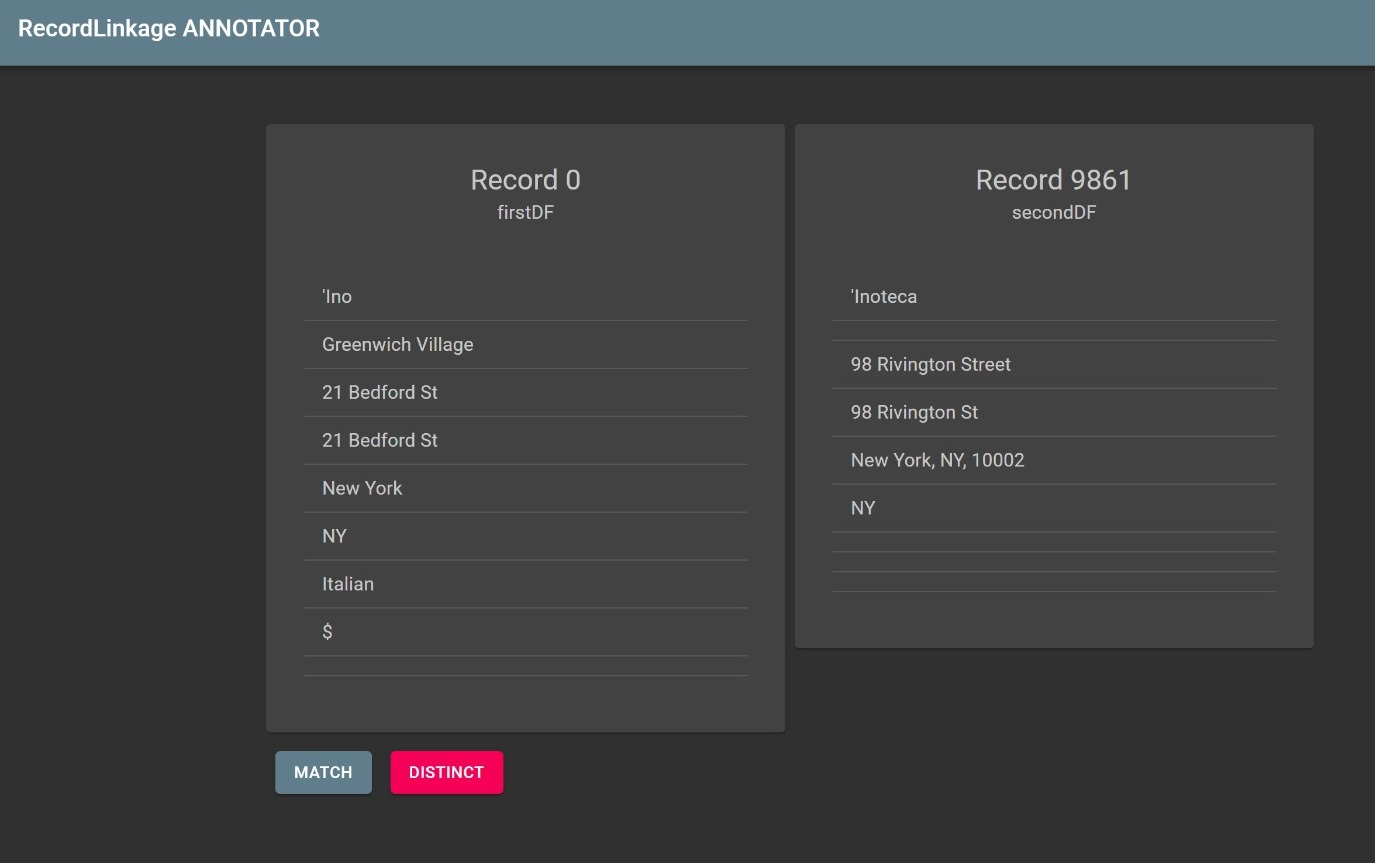
\includegraphics[width=0.8\linewidth]{img/match.jpeg}
	\caption{\textit{Interfaccia web per la classificazione manuale}}
\end{figure}

Nell'esempio che abbiamo appena fatto, possiamo notare come non ci sia nessun tipo di match in quanto nessuna delle informazioni presenti sono similari. \\
Quello che otteniamo alla fine sono 18 coppie che presentano match, % da capire se confronto va fatto con sottoinsieme coppie o no

\textbf{Risultati}: 
% non saprei che altro scrivere

\subsection{Gold Standard}
Il gold standard fornito è un elenco di 467 rimossi da alcuni siti web con l'informazione riguardante il suo stato al momento della verifica (Y = aperto, N = chiuso). 
% lo mettiamo? se lo mettiamo dobbiamo argomentare


% DA FARE:
% inserire e commentare immagine di pipeline di lavoro

% come facciamo a dire che siamo soddisfatti dell'integrazione dei DB, || PERCHè SI || Siamo soddisfatti perchè partendo da 7 file di testo contenenti in alcuni casi informazioni futili o assenti, attraverso la nostra operazione di pulizia dei dati, siamo riusciti a creaere due db che interagendo tra di loro forniscono delle info più che soddisfacenti. possiamo scrivere una cagata così
% partiamo dal fatto che rappresenta un caso reale, valutazione empirica.
% Con ECM probabilà 3 livelli di soglie,  || NON HO CAPITO by silvia || per ora non serve a un cazzo

\newpage
\printbibliography[title=Bibliografia]

\end{document}
